\documentclass[../main]{subfiles}
\begin{document}

\chapter{三点式正弦振荡器}%
\label{cha:三点式正弦振荡器}

\section{实验目的}%
\label{sec:\arabic{chapter}实验目的}

\begin{enumerate}

	\item 掌握三点式正弦波振荡器电路的基本原理,起振条件,振荡电路设计及电路
		参数计算。

	\item 通过实验掌握晶体管静态工作点、反馈系数大小对振荡幅度的影响。

\end{enumerate}

\section{基本原理}%
\label{sec:\arabic{chapter}基本原理}

\begin{figure}[htbp]
	\centering
	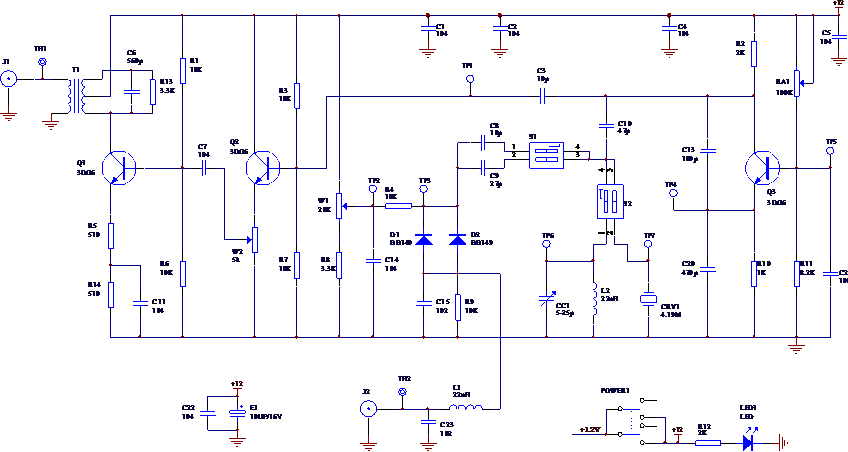
\includegraphics[width=0.8\linewidth]{circuit.png}
	\caption{正弦波振荡器}
	\label{fig:正弦波振荡器}
\end{figure}

将开关$S_3$拨上$S_4$拨下,$S_1$、$S_2$全部断开,由晶体管$Q_3$和$C_{13}$、
$C_{20}$、$C_{10}$、CCI、$L_2$构成电容反馈三点式振荡器的改进型振荡器--西勒振荡
器,电容CCI可用来改变振荡频率。

\begin{align}
	f_0 = \dfrac{1}{2\pi \sqrt{L_2(C_{10} + \mathrm{CCI})}}
\end{align}

振荡器的频率约为\SI{4.5}{\MHz}。

振荡电路反馈系数: $ F = \dfrac{C_{13}}{C_{20}} = \dfrac{56}{470} \approx 0.12 $

振荡器输出通过耦合电容$ C_3 = \SI{10}{\pF} $加到由$ Q_2 $组成的射极跟随器的输入
端,因 $ C_3 $ 容量很小,再加上射随器的输入阻抗很高,可以减小负载对振荡器的影响
。射随器输出信号 $ Q_1 $ 调谐放大,再经变压器耦合从$ J_1 $输出。

\section{实验步骤}%
\label{sec:\arabic{chapter}实验步骤}

根据图\ref{fig:正弦波振荡器}在实验板上找到振荡器各零件的位置并熟悉各元件的作用。

研究振荡器静态工作点对振荡幅度的影响。

将开关$ S_3 $拨上$ S_4 $拨下,$ S_1 $、$ S_2 $全拨下,构成LC振荡器。

\begin{figure}[htbp]
	\centering
	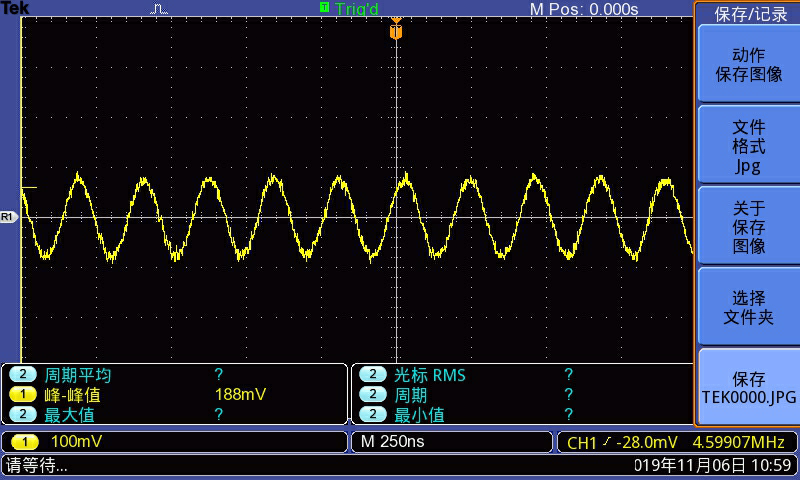
\includegraphics[width=0.8\linewidth]{LC.png}
	\caption{LC振荡器波形}
	\label{fig:LC振荡器波形}
\end{figure}

改变上偏置电位器$ \mathrm{RA}_1 $,记下发射极电流 ,并用示波器测量对应点的振荡幅
度 $ V_\mathrm{P-P} $(峰峰值)记下对应峰峰值以及停振时的静态工作点电流值。

\begin{table}[htbp]
	\centering
	\caption{峰峰值以及停振时的静态工作点电流值}
	\label{tab:峰峰值以及停振时的静态工作点电流值}
	\csvautobooktabular{tab/\arabic{chapter}/1.csv}
\end{table}

\begin{figure}[htbp]
	\centering
	\begin{subfigure}[htbp]{.45\linewidth}
		\centering
		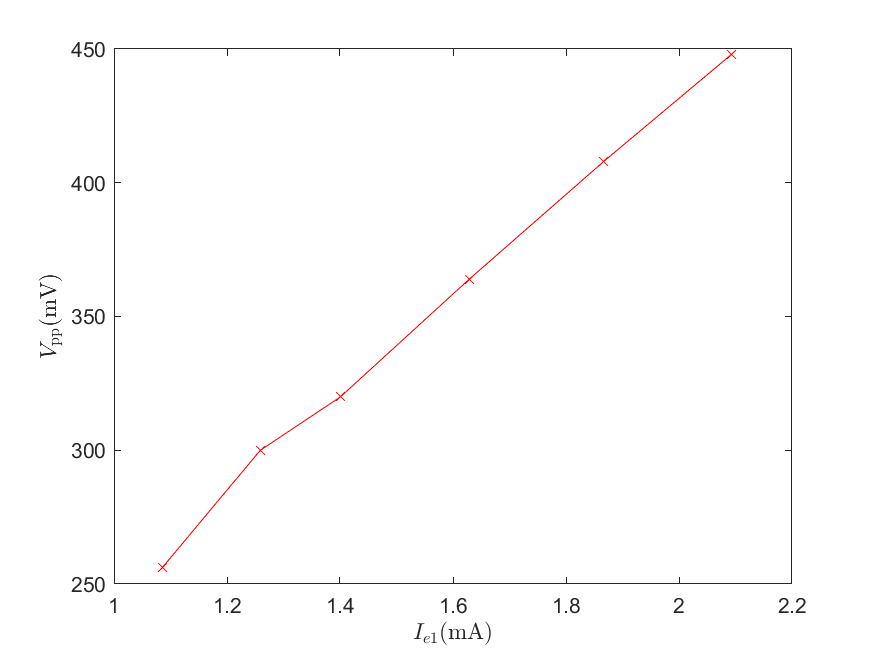
\includegraphics[width = \linewidth]{1-1.png}
		\caption{停振时的静态工作点电流值}
		\label{fig:停振时的静态工作点电流值}
	\end{subfigure}
	\quad
	\begin{subfigure}[htbp]{.45\linewidth}
		\centering
		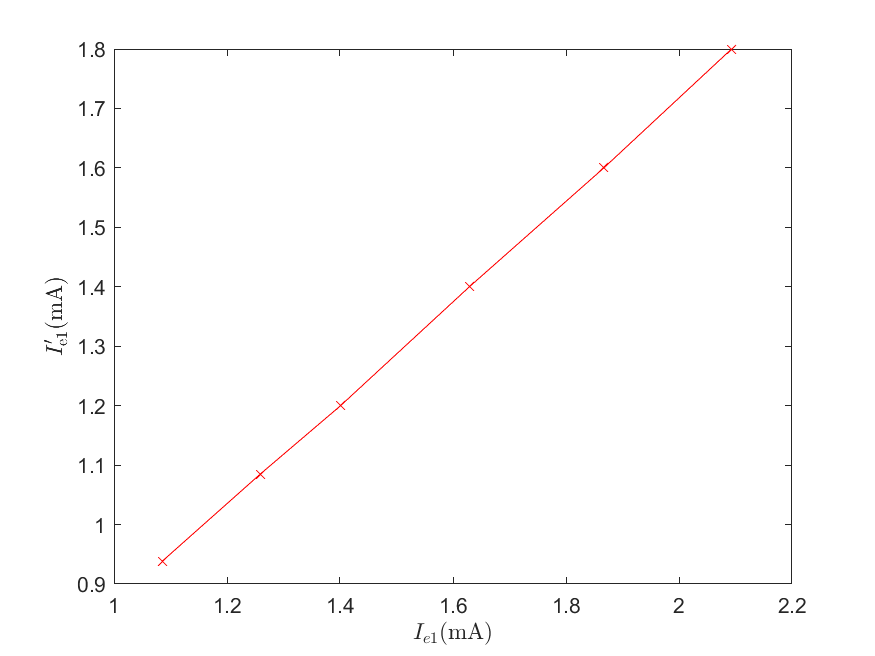
\includegraphics[width = \linewidth]{1-2.png}
		\caption{峰峰值}
		\label{fig:峰峰值}
	\end{subfigure}
	\caption{峰峰值以及停振时的静态工作点电流值}
	\label{fig:峰峰值以及停振时的静态工作点电流值}
\end{figure}

如图\ref{fig:震荡电压与静态工作点},分析输出振荡电压和振荡管静态工作点的关系,按
以上调整静态工作点的方法改变$ I_\mathrm{eq} $ ,并测量相应的 $ U_\mathrm{P - P}
$,且把数据记入表 \ref{tab:震荡电压与静态工作点关系} 。

\begin{table}[htbp]
	\centering
	\caption{震荡电压与静态工作点关系}
	\label{tab:震荡电压与静态工作点关系}
	\csvautobooktabular{tab/\arabic{chapter}/2.csv}
\end{table}

\begin{figure}[htbp]
	\centering
	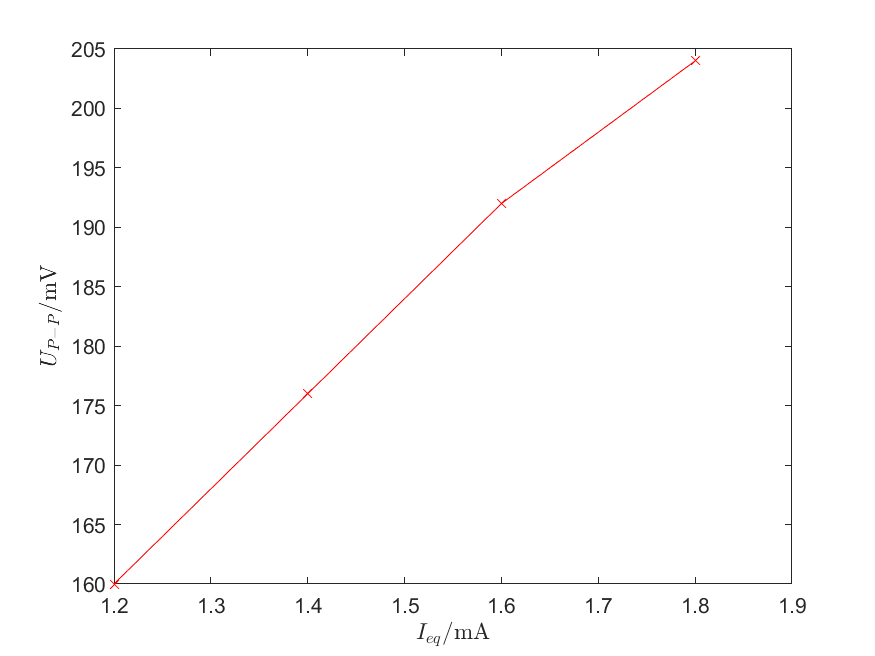
\includegraphics[width = 0.8\linewidth]{2-1.png}
	\caption{震荡电压与静态工作点关系}
	\label{fig:震荡电压与静态工作点关系}
\end{figure}

\begin{figure}[htbp]
	\centering
	\begin{subfigure}[htbp]{.45\linewidth}
		\centering
		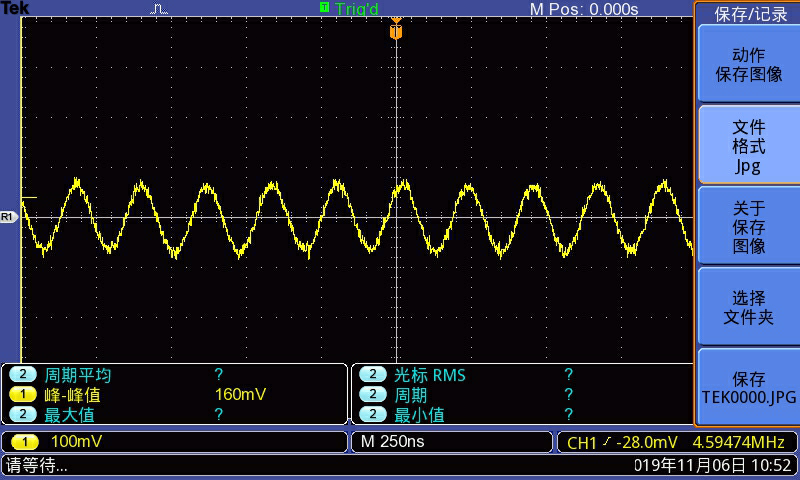
\includegraphics[width = \linewidth]{12.png}
		\caption{$I_\mathrm{e} = \SI{1.2}{\A}$}
		\label{fig:1.2}
	\end{subfigure}
	\quad
	\begin{subfigure}[htbp]{.45\linewidth}
		\centering
		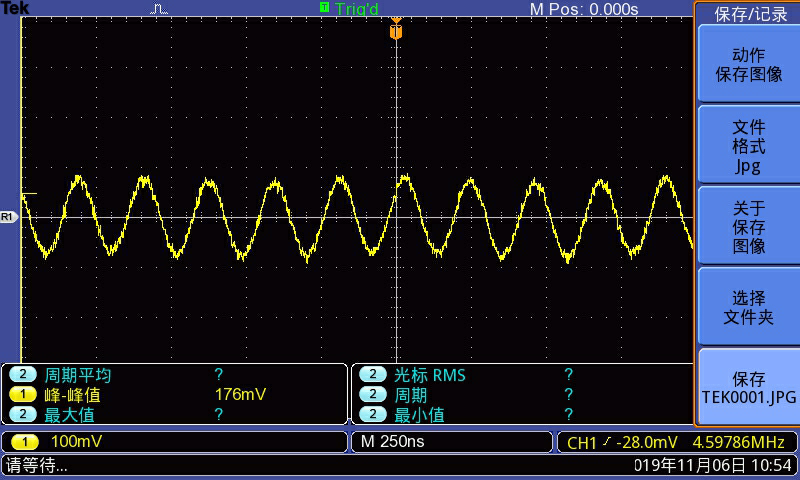
\includegraphics[width = \linewidth]{14.png}
		\caption{$I_\mathrm{e} = \SI{1.4}{\A}$}
		\label{fig:1.4}
	\end{subfigure}

	\begin{subfigure}[htbp]{.45\linewidth}
		\centering
		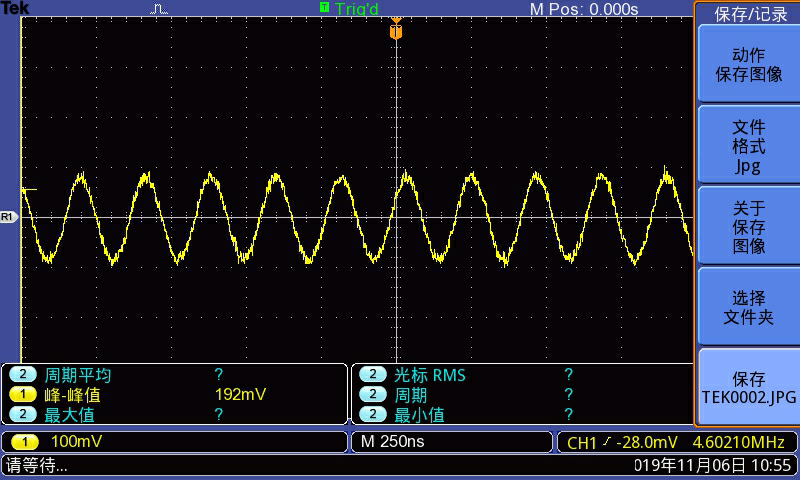
\includegraphics[width = \linewidth]{16.png}
		\caption{$I_\mathrm{e} = \SI{1.6}{\A}$}
		\label{fig:1.6}
	\end{subfigure}
	\quad
	\begin{subfigure}[htbp]{.45\linewidth}
		\centering
		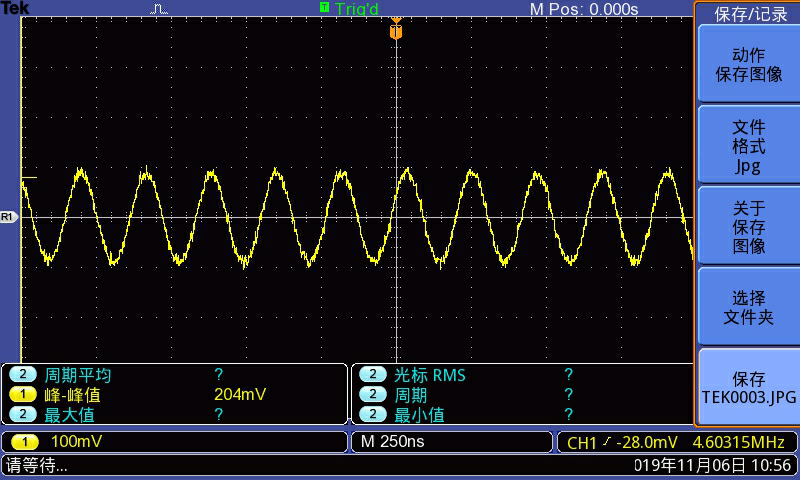
\includegraphics[width = \linewidth]{18.png}
		\caption{$I_\mathrm{e} = \SI{1.8}{\A}$}
		\label{fig:1.8}
	\end{subfigure}
	\caption{震荡电压与静态工作点}
	\label{fig:震荡电压与静态工作点}
\end{figure}

晶体振荡器:将开关$ S_4 $拨上$ S_3 $拨下,$ S_1 $、$ S_2 $全部拨下,由$ Q_3 $、$
C_{13} $、 $ C_{20} $、晶体 $ \mathrm{CRY}_1 $与 $ C_{10} $构成晶体振荡器(皮尔
斯振荡电路),在振荡频率上晶体等效为电感。

\begin{figure}[htbp]
	\centering
	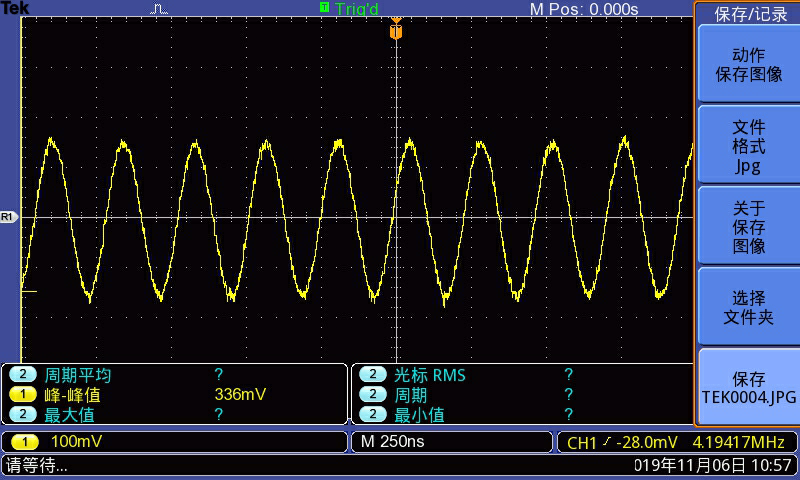
\includegraphics[width=0.6\linewidth]{oscilator.png}
	\caption{晶振波形}
	\label{fig:晶振波形}
\end{figure}

\section{实验报告要求}%
\label{sec:\arabic{chapter}实验报告要求}

\begin{Exercise}

	分析静态工作点、反馈系数$ F $对振荡器起振条件和输出波形振幅的影响,并用
	所学理论加以分析。

\end{Exercise}

\begin{Answer}

	由表\ref{tab:震荡电压与静态工作点关系}可以看出,当静态工作电流增大时,输
	出的振荡电压也随之增大。当反馈系数 $ F $增大时,输出的振荡电压减小,但输
	出波形振幅会更加稳定。

\end{Answer}

\section{实验仪器}%
\label{sec:\arabic{chapter}实验仪器}

\begin{table}[htbp]
	\centering
	\caption{实验仪器}
	\label{tab:\arabic{chapter}实验仪器}
	\csvautobooktabular{tab/\arabic{chapter}/BOM.csv}
\end{table}

\end{document}

